% Implication graph of the seven 2-clauses of Chapter 1's opening question (generated by a script).
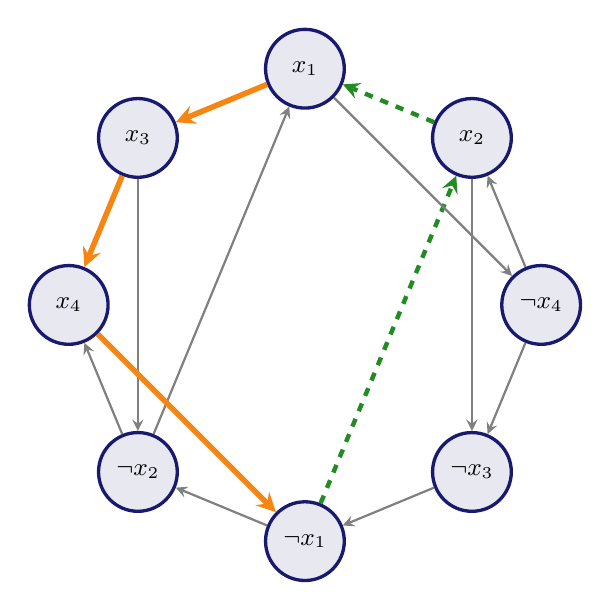
\begin{tikzpicture}[>=stealth,lit/.style={circle,draw=MidnightBlue,very thick,fill=MidnightBlue!10,minimum size=10mm,inner sep=0pt,font=\small}]
\node[lit] (p1) at (0.000,3.000) {$x_1$};
\node[lit] (p3) at (-2.121,2.121) {$x_3$};
\node[lit] (p4) at (-3.000,0.000) {$x_4$};
\node[lit] (n2) at (-2.121,-2.121) {$\neg x_2$};
\node[lit] (n1) at (-0.000,-3.000) {$\neg x_1$};
\node[lit] (n3) at (2.121,-2.121) {$\neg x_3$};
\node[lit] (n4) at (3.000,-0.000) {$\neg x_4$};
\node[lit] (p2) at (2.121,2.121) {$x_2$};
\draw[->,thick,gray] (n4) -- (n3);
\draw[->,thick,gray] (n4) -- (p2);
\draw[->,thick,gray] (n3) -- (n1);
\draw[->,thick,gray] (n2) -- (p1);
\draw[->,thick,gray] (n2) -- (p4);
\draw[->,thick,gray] (n1) -- (n2);
\draw[->,line width=1.6pt,dashed,ForestGreen] (n1) -- (p2);
\draw[->,thick,gray] (p1) -- (n4);
\draw[->,line width=2pt,BurntOrange] (p1) -- (p3);
\draw[->,thick,gray] (p2) -- (n3);
\draw[->,line width=1.6pt,dashed,ForestGreen] (p2) -- (p1);
\draw[->,thick,gray] (p3) -- (n2);
\draw[->,line width=2pt,BurntOrange] (p3) -- (p4);
\draw[->,line width=2pt,BurntOrange] (p4) -- (n1);
\end{tikzpicture}
